\documentclass[10pt]{beamer}

% Beamer style
%\usetheme[secheader]{Madrid}
% \usetheme{CambridgeUS}
\useoutertheme{infolines}
\usecolortheme[rgb={0.65,0.15,0.25}]{structure}
% \usefonttheme[onlymath]{serif}
\beamertemplatenavigationsymbolsempty
%\AtBeginSubsection

% Packages
%\usepackage[french]{babel}
\usepackage[latin1]{inputenc}
\usepackage{color}
\usepackage{xspace}
%\usepackage{dsfont, stmaryrd}
\usepackage{amsmath, amsfonts, amssymb}
\usepackage{epsfig}
\usepackage{url}
\usepackage{/home/robin/LATEX/Biblio/astats}
%\usepackage[all]{xy}
\usepackage{graphicx}

% Commands
\definecolor{darkred}{rgb}{0.65,0.15,0.25}
\newcommand{\emphase}[1]{\textcolor{darkred}{#1}}
% \newcommand{\emphase}[1]{{#1}}
\newcommand{\paragraph}[1]{\textcolor{darkred}{#1}}
\newcommand{\refer}[1]{{\footnotesize{\textcolor{gray}{[{\cite{#1}}]}}}}
\newcommand{\Refer}[1]{{\footnotesize{\textcolor{gray}{[{#1}]}}}}
\renewcommand{\newblock}{}

% Symbols
\newcommand{\BM}{\text{BM}}
\newcommand{\dd}{\xspace\text{d}}
\newcommand{\Esp}{\mathbb{E}}
\newcommand{\Ibb}{\mathbb{I}}
\newcommand{\Cov}{\mathbb{C}\text{ov}}
\newcommand{\OU}{\text{OU}}
\newcommand{\Var}{\mathbb{V}}
\newcommand{\Hcal}{\mathcal{H}}
\newcommand{\Mcal}{\mathcal{M}}
\newcommand{\Ncal}{\mathcal{N}}
\newcommand{\pa}{\text{pa}}
\newcommand{\ra}{\emphase{\mathversion{bold}{$\rightarrow$}~}}
\newcommand{\Scal}{\mathcal{S}}

% Directory
\newcommand{\fig}{../FIGURES}
%\newcommand{\figmotif}{/home/robin/RECHERCHE/RESEAUX/Motifs/FIGURES}


%====================================================================
%====================================================================

%====================================================================
%====================================================================
\begin{document}
%====================================================================
%====================================================================

%====================================================================
\title[Detection of adaptive shifts]{Detection of adaptive shifts on phylogenies using shifted stochastic processes on a tree}

\author[S. Robin]{P. Bastide, M. Mariadassou, \underline{S. Robin} + C. An�}

\institute[INRA/AgroParisTech/Paris-Saclay]{% INRA / AgroParisTech \\ ~\\
%  \vspace{-.1\textwidth}
  \begin{tabular}{ccccc}
    
\includegraphics[height=.06\textheight]{\fig/LogoINRA-Couleur} & 
    \hspace{.02\textheight} &
    
\includegraphics[height=.06\textheight]{\fig/logagroptechsolo} & 
    \hspace{.02\textheight} &
    
\includegraphics[height=.0633\textheight]{\fig/LogoParisSaclay}
    \\ 
  \end{tabular} \\
  \bigskip
  }

\date[Copenhagen, 2017]{Nordic-Baltic Biometric Conference, Copenhagen, June 2017}

%====================================================================
%====================================================================
\maketitle
%====================================================================

%====================================================================
%====================================================================
\section{Modeling adaptive shifts}
\frame{\frametitle{Outline} \tableofcontents[currentsection]}
%====================================================================
\frame{\frametitle{Diversity of a trait}

  The diversity of a trait among a set of species results from:
  \begin{itemize}
   \item their shared history,
   \item potential %isolated shifts corresponding to 
   adaptive shifts due, e.g. to changes of ecological niche.
  \end{itemize}
  $$
  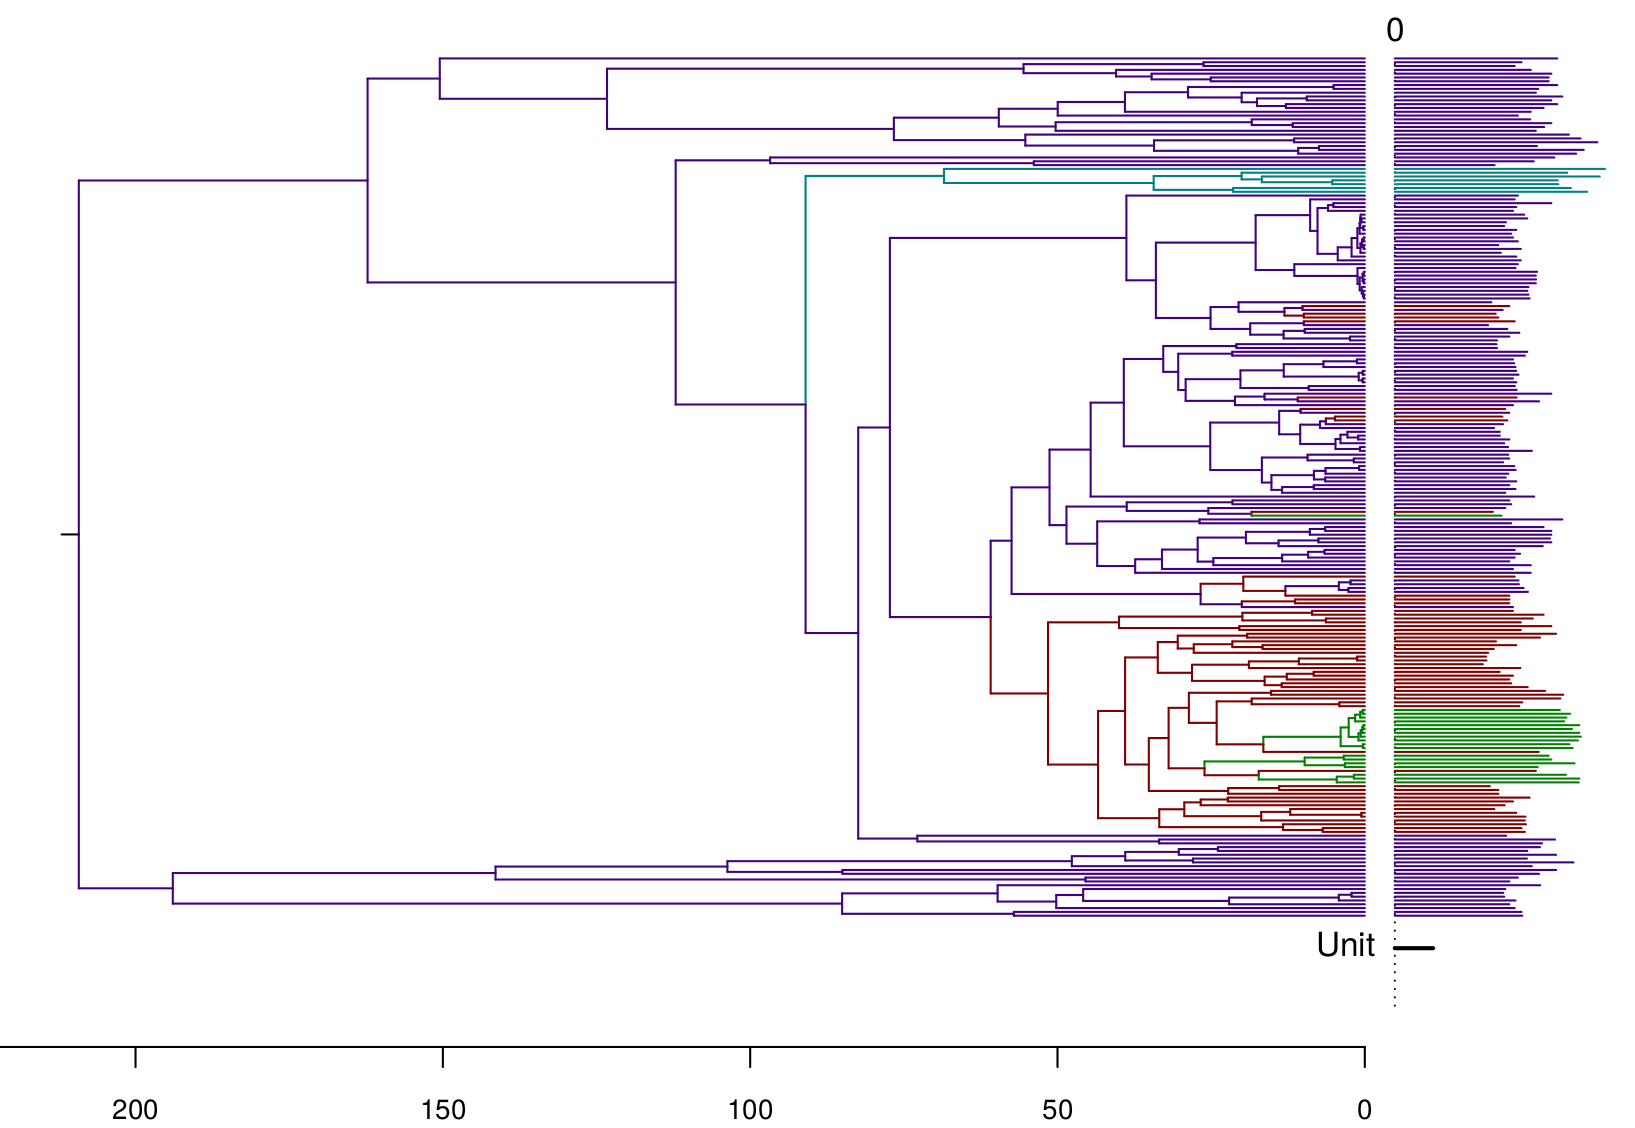
\includegraphics[width=.6\textwidth, clip=]{../FIGURES/plot_data_chel-intro-SR}
  $$
  \refer{JSA11}: Turtle species Trait: carapace length 
  }

%====================================================================
\frame{\frametitle{Evolution of a trait}

  \begin{tabular}{cc}
    \begin{tabular}{p{.5\textwidth}}	
    Phylogenetic tree \\
    \vspace{-.15\textheight}
    \includegraphics[width=.5\textwidth, clip=]{../FIGURES/plot_tree_tims_2-1}
    \\
    \vspace{-.1\textheight}
    \onslide+<2->{
	 Process on the tree  \\
	 \vspace{-.15\textheight}
	 \includegraphics[width=.5\textwidth, clip=]{../FIGURES/plot_BM_sim_2-1}
	 }
    \end{tabular}
    &    
    \hspace{-.1\textwidth}
    \begin{tabular}{p{.45\textwidth}}
    \paragraph{Model for trait $X$:} no cluster\\ ~
    \begin{itemize}
    \onslide+<2->{
	 \item $X$ is a random process (e.g. Brownian motion = BM) that goes along the
	 branches of the tree \refer{Fel85}; \\ ~
	 \item at each internal nodes, independent copies of the processes bifurcate; \\ ~
    }
    \onslide+<3->{
	 \item only the leafs $Y_1, Y_2, \dots Y_n$ are observed: 
	 \begin{eqnarray*}
	 \text{for BM:} \quad 
	 \Var(X_A|R) & = & \sigma^2 t, \\
	 \Cov(X_A, X_B|R) & = & \sigma^2 t_{AB},
	 \end{eqnarray*}
	 }
    \end{itemize} \\
    \end{tabular}
  \end{tabular}
  }

%====================================================================
\frame{\frametitle{Introducing shifts}

  \begin{tabular}{cc}
    \begin{tabular}{p{.5\textwidth}}	
    Phylogenetic tree \\
    \vspace{-.15\textheight}
    \includegraphics[width=.5\textwidth, clip=]{../FIGURES/plot_tree_tims_shift-1}
    \\
    \vspace{-.1\textheight}
    \onslide+<2->{
	 Process on the tree  \\
	 \vspace{-.15\textheight}
	 \includegraphics[width=.5\textwidth, clip=]{../FIGURES/plot_BM_sim_shit-1} \\
	 clusters: $(A, B, D)$ / $(C, E)$
    }
    \end{tabular}
    &    
    \hspace{-.1\textwidth}
    \begin{tabular}{p{.45\textwidth}}
    \paragraph{Model with $K$ shifts:} clusters\\ ~
    \begin{itemize}
    \onslide+<2->{
	 \item Same model as before; \\ ~
	 \item at the start of $K$ branches $\tau_k$, shifts (with magnitude $\delta_k$;) occur; \\ ~
    }
    \onslide+<3->{
	 \item the distribution of the process is shifted accordingly: \\
	 for BM
	 \begin{eqnarray*}
	 \mu_j & = & \mu_{\pa(j)} + \sum_k \delta_k \mathbb{I}\{\tau_k=b_j\},
	 \end{eqnarray*}
    }
    \end{itemize} \\ ~\\ ~\\ ~\\
  \end{tabular}
  \end{tabular}
}

%====================================================================
\frame{\frametitle{Ornstein-Uhlenbeck model}

  \paragraph{Brownian motion:} $\dd X(t) = \sigma \dd W(t)$ 
  \begin{itemize}
   \item Easy to handle (no memory);
   \item Not realistic: no stationary distribution \ra the trait can wander anywhere.
  \end{itemize}

  \bigskip \bigskip \pause
  \paragraph{Ornstein-Uhlenbeck (OU):} 
  \begin{itemize}
   \item Solution of   
   $$
   \dd X(t) = \sigma \dd W(t) - \alpha \left(X(t) - \beta\right) \dd t
   $$
   Recall with strength $\alpha$ toward an $\beta$;
%    Continuous counterpart of an $AR(1)$ time series;
   \item More realistic: has stationary distribution 
   $$
   \Ncal(\beta, \gamma^2), \qquad \gamma^2 = \sigma^2/2\alpha,
   $$
   $\beta =$ 'optimum' value for the trait \refer{Han97,BuK04}.
  \end{itemize} 
}

%====================================================================
\frame{\frametitle{Ornstein-Uhlenbeck model with shifts}

  \paragraph{Adaptive shift:} Due to some variation of the environment, a shift occurs in $\beta$:
  \vspace{-.1\textheight}
  $$
%   \vspace{-.1\textheight}
  \includegraphics[width=.7\textwidth]{../FIGURES/plot_OU_sim_shit-1}
  $$
  $$
  X_i | X_{\pa(i)} \sim \Ncal\left(X_{\pa(i)}e^{-\alpha \ell_i} + \beta_{i}(1 - e^{-\alpha \ell_i}), \frac{\sigma^2}{2\alpha} (1 - e^{-2\alpha \ell_i})\right)
  $$
}

%====================================================================
\frame{\frametitle{Reparametrization of the Ornstein-Uhlenbeck model}

  \paragraph{Property.} $X(t) =$ Ornstein-Uhlenbeck process, $W(t) = $ Brownian motion:
  $$
  X(t) = \sigma e^{-\alpha t} W(e^{2 \alpha t} - 1) / \sqrt{2 \alpha}
  $$
  
  
  \bigskip \bigskip \pause
  \paragraph{Consequence.} If $T$ is ultra-metric, we have 
  $$
  p_{\emphase{\OU}, \alpha}(Y_1, \dots Y_n; T) = p_{\emphase{\BM}}(Y_1, \dots Y_n; \emphase{\widetilde{T}})
  $$
  where $\widetilde{T}$ is the rescaled tree with branch lengths
  $$
  \ell(\alpha) =  \frac{1}{2\alpha} e^{2-\alpha h} (e^{2\alpha t_i} - e^{2\alpha t_\pa(i)})
  $$
}

%====================================================================
%====================================================================
\section{Inference}
\frame{\frametitle{Outline} \tableofcontents[currentsection]}
%====================================================================

%====================================================================
\frame{\frametitle{V1: Incomplete data model}

%   \hspace{-.055\textwidth}
  \paragraph{Complete data} $X = (Z, Y)$
  \begin{itemize}
  \item $(Z_i) = $ traits at the internal nodes (ancestors);
  \item $(Y_j) = $ traits at the leafs (extant species).
  \end{itemize}

  $$
  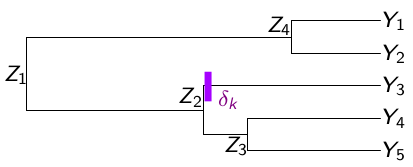
\includegraphics[width=.6\textwidth]{../FIGURES/IncompleteData-BMR15}
  $$
  
  \bigskip \bigskip 
  \ra Standard inference algorithm = EM \refer{DLR77}
  }

%====================================================================
\frame{\frametitle{V1: EM algorithm}

  \paragraph{E-step.} 2 ways to compute $p_{\theta^h}(X \; | \; Y)$
  \begin{enumerate}
   \item General properties of multivariate Gaussian (+ \refer{HoA13b}'s trick to invert $S_{YY}$).
   \item \emphase{Upward-downward} recursion taking advantage of the tree structure.
  \end{enumerate}
  
  \bigskip \bigskip \bigskip \pause
  \paragraph{M-step.} The update of $\theta^h$ include the \emphase{optimal allocation} of shifts to branches. Two costs to compare for each branch
  \begin{eqnarray*}
   \text{without shift:} & & \Esp [\log \phi(X_j; X_{pa(j)}, \ell_j \sigma^2) | Y]\\
   \text{with shift:} & & \Esp [\log \phi(X_j; X_{pa(j)} \emphase{+ \delta_k}, \ell_j \sigma^2) | Y]
  \end{eqnarray*}
  \ra Trivial optimal allocation problem.
}

%====================================================================
\frame{\frametitle{V2: Regression model}

  \begin{tabular}{cc}
    \begin{tabular}{p{.5\textwidth}}
	 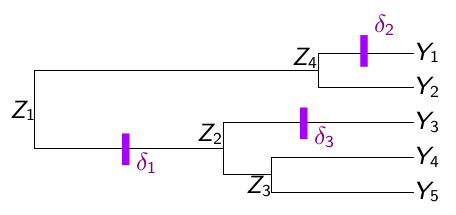
\includegraphics[width=.5\textwidth]{../FIGURES/RegressionView-BMR15}
    \end{tabular}
    & 
    \hspace{-.1\textwidth}
    \begin{tabular}{p{.5\textwidth}}
    {\scriptsize
    \[
    \Delta = \begin{bmatrix}
	 \mu\\ \delta_1\\ 0\\  0\\ \delta_2\\ 0\\ \delta_3\\ 0\\ 0\\
    \end{bmatrix}                           
    \qquad 
    T \Delta = \begin{bmatrix}
	 \mu + \delta_2\\ \mu\\ \mu + \delta_1 + \delta_3\\ \mu + \delta_1\\ \mu + \delta_1\\ 
    \end{bmatrix}
    \]
    }
    \end{tabular} 
    \\
    \begin{tabular}{p{.5\textwidth}}
         {\scriptsize
         \[
         \!\!\!T\!=\!
         \bordermatrix{
         \!&Z_1\!\!\!&Z_2\!\!\!&Z_3\!\!\!&Z_4\!\!\!&\!\!\!&Y_1\!\!\!&Y_2\!\!\!&Y_3\
         \!\!&Y_4\!\!\!&Y_5\cr
         Y_1\!&1&0&0&1&\!\!\!&1&0&0&0&0 \cr
         Y_2\!&1&0&0&1&\!\!\!&0&1&0&0&0 \cr
         Y_3\!&1&1&0&0&\!\!\!&0&0&1&0&0 \cr
         Y_4\!&1&1&1&0&\!\!\!&0&0&0&1&0 \cr
         Y_5\!&1&1&1&0&\!\!\!&0&0&0&0&1 \cr 
         }\]
         }
    \end{tabular}
    & 
    \hspace{-.1\textwidth}
    \begin{tabular}{p{.5\textwidth}}
    \begin{eqnarray*}
    Y & = & T\Delta + E \\
    E  & \sim & \Ncal(0, \Sigma) \\
    ~\\
    ( \Sigma & = & S_{YY})
    \end{eqnarray*}
    \end{tabular}
  \end{tabular}

  }

% %====================================================================
% \frame{\frametitle{Some more about the inference}
% 
%   \paragraph{Regression point of view:}
%   \begin{itemize}
%    \item Lasso initialization: 
%    $$
%    \arg\min_\delta \|Y - T\Delta\|^2_{\Sigma^{-1}} + \lambda |\Delta|;
%    $$
%    \item Identifiability issues: the null space of $T$ does not reduce to $0$;
%    \item Useful representation for model selection.
%   \end{itemize}
% 
%   \bigskip \pause
%   \paragraph{Ornstein-Uhlenbeck:} 
%   \begin{itemize}
%    \item Regression version
%    $$
%    Y = T W(\alpha) \Delta + E, \qquad E \sim \Ncal(0, \Sigma(\alpha))
%    $$
%    \ra Lasso intialization, identifiability and model selection still holds.
%    \item Estimation of $\alpha$: 
%    Either within the EM loop, or externally, using a grid.
%   \end{itemize}
% 
% }
% 
%====================================================================
%====================================================================
\section{Identifiability}
\frame{\frametitle{Outline} \tableofcontents[currentsection]}
%====================================================================
\frame{\frametitle{Identifiability}

  \begin{itemize}
   \item Shift allocation results in a coloring of the leafs (observable);
   \onslide+<2->{\item Some scenarios are parsimonious, some are not (homoplasy).}
   \onslide+<4->{\item Different scenarios may results in the same coloring.}
  \end{itemize}
  
  \begin{overprint}
   \onslide<3>
     \begin{tabular}{p{.25\textwidth}p{.05\textwidth}p{.25\textwidth}p{.05\textwidth}p{.25\textwidth}}
	 \begin{tabular}{c}
	 \includegraphics[width=0.15\textwidth]{../FIGURES/colours_1_nodes_gray} \\
	 2 colors \\ ~
	 \end{tabular}
	 & 
	 \begin{tabular}{c}
	 $:$
	 \end{tabular}
	 & 
	 \begin{tabular}{c}
	 \includegraphics[width=0.15\textwidth]{../FIGURES/colours_2_nodes_gray} \\
	 non \\
	 parsimonious
	 \end{tabular}
	 & 
	 \begin{tabular}{c}
	 $<$
	 \end{tabular}
	 & 
	 \begin{tabular}{c}
	 \includegraphics[width=0.15\textwidth]{../FIGURES/colours_3_nodes_gray} \\
	 parsimonious \\ ~
	\end{tabular}
  \end{tabular}
  \onslide<5>
     \begin{tabular}{p{.25\textwidth}p{.05\textwidth}p{.25\textwidth}p{.05\textwidth}p{.25\textwidth}}
	 \begin{tabular}{c}
	 \includegraphics[width=0.15\textwidth]{../FIGURES/colours_bis_1_nodes_gray} \\
	 3 colors
	 \end{tabular}
	 & 
	 \begin{tabular}{c}
	 $:$
	 \end{tabular}
	 & 
	 \begin{tabular}{c}
	 \includegraphics[width=0.15\textwidth]{../FIGURES/colours_bis_2_nodes_gray} \\
	 parsimonious
	 \end{tabular}
	 & 
	 \begin{tabular}{c}
	 $\sim$
	 \end{tabular}
	 & 
	 \begin{tabular}{c}
	 \includegraphics[width=0.15\textwidth]{../FIGURES/colours_bis_3_nodes_gray} \\
	 parsimonious
	\end{tabular}
  \end{tabular}
  \end{overprint}
}

%====================================================================
\frame{ \frametitle{Models with $K$ shifts}

  \paragraph{No homoplasy:} 1 shift = 1 new color.
  $$
  K \text{ shifts} \quad \Leftrightarrow \quad K + 1 \text{ colors}
  $$
 
  \bigskip \pause
  \paragraph{Actual number of models:}
  \begin{align*}
  \Scal_K^{PI} &= \Scal_K^{P}/\sim; \\
  \Scal_K^P & = \{\text{Parsimonious allocations of $K$ shifts}\} %\\
%   \Scal_K^{PI} & \simeq \{\text{Tree compatible coloring of tips in $K+1$ colors}\} 
  \end{align*}
  \ra Complexity of the $K$-shifts model class $= \# \Scal_K^{PI}$
  
  \pause \bigskip \bigskip
  \paragraph{Problem:}
  $$
  \# \Scal_K^{PI} = ?
  $$
}

%====================================================================
\frame{ \frametitle{Number of models with $K$ shifts}

  $\#{\Scal_K^{PI}}$ depends on the topology of the tree.

  \bigskip \bigskip \pause
  \paragraph{Some new results:}
  \begin{enumerate}
  \item $\#{\Scal_K^{PI}}$ can be computed recursively \refer{BMR16}. In any cases,
  $$
  \#{\Scal_K^{PI}} \leq \binom{m+n-1}{K}
  $$
  \item For a binary tree: 
  $$
  \#{\Scal_K^{PI}} = \binom{2n-2-K}{K}.
  $$
  \item Parsimonious equivalent scenarios can be enumerated (generalization of \refer{Fel04}.)
  \end{enumerate}

}

%====================================================================
\frame{ \frametitle{Example of equivalent scenarios}

  OU model: this 5 configurations only count for 1.
  $$
  \includegraphics[width=.8\textwidth]{../FIGURES/plot_parsimony-1}
  $$
}

%====================================================================
\frame{ \frametitle{Model selection: $K =$?}

  \paragraph{Specificity:} due to the discrete nature of the shift locations, standard criteria (AIC, BIC) do not apply.
  
  \bigskip \bigskip \pause
  \paragraph{Penalized criterion.} Under the BM model $Y = T \Delta + E$, $E \sim \Ncal(0, \Sigma)$, taking
  $$
  \widehat{\eta} = \arg\min_{\eta \in \Mcal} \|Y - \widehat{s}_\eta\|^2_{\Sigma^{-1}} + (1 + \text{Pen}(K_\eta))
  $$
  where
  $$
  \Mcal = \bigcup_{K \geq 0} \Scal^{PI}_K, 
  \qquad
  \text{Pen}(K) = f(n, K, \# \Scal^{PI}_K)
  $$
  \pause ensures the oracle inequality
  $$
  \|Y - \widehat{s}_{\widehat{\eta}}\|^2_{\Sigma^{-1}}
  \leq C_1 \left(\inf_{\eta \in \Mcal} \|s - \widehat{s}_\eta\|^2_{\Sigma^{-1}} + C_2(n, \eta) + C_3(n) \right)
  $$
  
  \paragraph{Proof.} Adaptation of \refer{BGH09}. 
}

%====================================================================
%====================================================================
\section{Illustration}
\frame{\frametitle{Outline} \tableofcontents[currentsection]}
%====================================================================

% %====================================================================
% \frame{ \frametitle{Some simulations}
% 
%   \begin{overprint}
%     \onslide<1>
%     \paragraph{An example:} left: simulated, right: estimated (3 equivalent scenarios)
%     $$  
%     \includegraphics[width=\textwidth]{../FIGURES/plot_est_eqs-1} 
%     $$
%     \onslide<2>
%     \vspace{-.1\textheight}
%     $$
%     \includegraphics[width=\textwidth]{../FIGURES/plot_simus_beta_0_K_ARI-1}
%     $$
%     \onslide<3>
%     \vspace{-.1\textheight}
%     $$
%     \includegraphics[width=\textwidth]{../FIGURES/plot_simus_LL_alpha_gamma-1}
%     $$
%   \end{overprint}
% }
% 
%====================================================================
\frame{ \frametitle{Chelonia turtles}

  \only<1>{
\begin{columns}
\begin{column}{0.55\textwidth}
\begin{minipage}[c][\textheight][c]{\linewidth}
\vskip -1 cm
    \includegraphics[width=\linewidth]{../FIGURES/plot_chel_data1-1} \\
    {\footnotesize Colors: habitats.\\ Boxes: selected EM regimes.}
\end{minipage}
\end{column}
\begin{column}{0.45\textwidth}
\begin{minipage}[t][.6\textheight][c]{\linewidth}
\end{minipage}
\end{column}
\end{columns}
}
\only<2>{
\begin{columns}
\begin{column}{0.55\textwidth}
\begin{minipage}[c][\textheight][c]{\linewidth}
\vskip -1 cm
    \includegraphics[width=\linewidth]{../FIGURES/plot_chel_data-1} \\
    {\footnotesize Colors: habitats.\\ Boxes: selected EM regimes.}
\end{minipage}
\end{column}
\begin{column}{0.45\textwidth}
\begin{minipage}[t][.6\textheight][c]{\linewidth}
\vskip - 4 cm
\includegraphics[width=0.5\textwidth]{../FIGURES/Chelonia_mydas.jpg} \\
{\footnotesize Chelonia mydas}
\end{minipage}
\end{column}
\end{columns}
}
\only<3>{
\begin{columns}
\begin{column}{0.55\textwidth}
\begin{minipage}[c][\textheight][c]{\linewidth}
\vskip -1 cm
\includegraphics[width=\linewidth]{../FIGURES/plot_chel_data3-1}  \\
{\footnotesize Colors: habitats.\\ Boxes: selected EM regimes.}
\end{minipage}
\end{column}
\begin{column}{0.45\textwidth}
\begin{minipage}[t][.6\textheight][c]{\linewidth}
\includegraphics[width=0.5\textwidth]{../FIGURES/Geochelone_nigra_abingdoni.jpg} \\
{\footnotesize Geochelone nigra abingdoni}
\end{minipage}
\end{column}
\end{columns}
}
\only<4>{
\begin{columns}
\begin{column}{0.55\textwidth}
\begin{minipage}[c][\textheight][c]{\linewidth}
\vskip -1 cm
\includegraphics[width=\linewidth]{../FIGURES/plot_chel_data5-1} \\
{\footnotesize Colors: habitats.\\ Boxes: selected EM regimes.}
\end{minipage}
\end{column}
\begin{column}{0.45\textwidth}
\begin{minipage}[t][.6\textheight][c]{\linewidth}
\vskip - 4 cm
\includegraphics[width=0.5\textwidth]{../FIGURES/Dudhwalive_chitra.jpg} \\
{\footnotesize Chitra indica}
\end{minipage}
\end{column}
\end{columns}
}
\only<5>{
\begin{columns}
\begin{column}{0.55\textwidth}
\begin{minipage}[c][\textheight][c]{\linewidth}
\vskip -1 cm
\hspace{.025\textwidth}
\includegraphics[width=\linewidth]{../FIGURES/plot_chel_data4-1} \\
{\footnotesize Colors: habitats.\\ Boxes: selected EM regimes.}
\end{minipage}
\end{column}
\begin{column}{0.5\textwidth}
\begin{minipage}[t][.6\textheight][c]{\linewidth}
\vskip - 3 cm
{\footnotesize
\begin{table}[!ht]
\begin{center}
\begin{tabular}{l|c|c}
\hline
  & Habitat & EM\\ \hline
Nb shifts & 16 & 5\\ \hline
Nb regimes & 4 & 6\\ \hline
$\log P$ & -135.56 & -97.59\\ \hline
$\ln 2 / \alpha$ (\%) & 7.83 & 5.43\\ \hline
$\gamma^2$ & 0.35 & 0.22\\ \hline
CPU (mn) & 1.25 & 134.49\\ \hline
\end{tabular}
\end{center}
\end{table}
}
\end{minipage}
\end{column}
\end{columns}
}
}

%====================================================================
%====================================================================
\section{Extension to multivariate traits}
\frame{\frametitle{Outline} \tableofcontents[currentsection]}
%====================================================================
%====================================================================
\frame{\frametitle{Multivariate OU model}

  \paragraph{Data.} ${\bf X}_j = (X_{j1}, \dots X_{jp})$, possibly correlated (${\bf R}$).
  
  \bigskip \bigskip \pause
  \paragraph{Multivariate OU model ${\bf X}(t)$.} ${\bf W}(t) =$ standard multivariate BM:
  $$
  \dd {\bf X}(t) = {\bf A}(\text{\mathversion{bold}{$\beta$}} - {\bf X}(t)) \dd t + {\bf R} \; \dd {\bf W}(t)
  $$
  where $\bf{A} = \alpha \mathbf{I}$ \ra 'scalar' OU (scOU) model \refer{BAR17}.
  
  \bigskip \bigskip \pause
  \paragraph{Some comments.} 
  \begin{itemize}
%    \item Tractable inference if ${\bf A}$ and ${\bf R}$ commute.
   \item scOU: same 'recall' to the optimum for all traits (but arbitrary ${\bf R}$)
   \item $\ell1$ou \refer{KKR16}: arbitrary ${\bf A}$ but independent traits (${\bf R}$ diagonal)
   \item Preliminary pPCA \refer{Rev09} does not remove correlation \emphase{in presence of shifts}
   \item Preliminary de-correlation is still useful for numerical reasons
  \end{itemize}
}

%====================================================================
\frame{\frametitle{\url{PhylogeneticEM} package}

  \paragraph{Monkey dataset.}
  \begin{itemize}
  \item {\tt res <- PhyloEM(Y\_data = ..., phylo = ..., process = "scOU", K\_max = 10, nbr\_alpha = 4, ...)} 
  \item {\tt plot(res, ...)}
  \end{itemize}
  $$
  \includegraphics[height=.6\textheight]{../FIGURES/BAM17-SupMat-Fig2}
  $$
}

%====================================================================
\frame{\frametitle{\url{PhylogeneticEM} package}

  \paragraph{Monkey dataset.}
  \begin{itemize}
  \item {\tt eq\_shifts <- equivalent\_shifts(phylogeny, params\_5)} 
  \item {\tt plot(eq\_shifts, ...)}
  \end{itemize}
  
  $$
  \includegraphics[width=.9\textwidth]{../FIGURES/BAM17-SupMat-Fig3}
  $$
}

%====================================================================
\frame{\frametitle{Conclusion \& Future works}

  \paragraph{Conclusions.}
  \begin{itemize}
   \item Comprehensive estimation framework: EM algorithm + identifiability + model selection;
   \item JRSS-B paper: \refer{BMR16}
   \item Extension to correlated multivariate traits: \refer{BAR17}
   \item R package \url{Phylogenetic-EM}.
  \end{itemize}

  \bigskip \bigskip \pause
  \paragraph{Future work.}
  \begin{itemize}
%    \item 'Spasify' the multivariate version so that not all traits are affected by each shift;
   \item Deal with the uncertainty of the tree;
   \item Consider fossil records to distinguish between equivalent scenarios.
  \end{itemize}

}

%====================================================================
\frame[allowframebreaks]{ \frametitle{References}

\nocite{BMR16,BAR17}

{\tiny
  \bibliography{/home/robin/Biblio/BibGene}
%   \bibliographystyle{/home/robin/LATEX/Biblio/astats}
  \bibliographystyle{alpha}
  }
}

%====================================================================
\frame{\frametitle{Notations}
  
  $$
  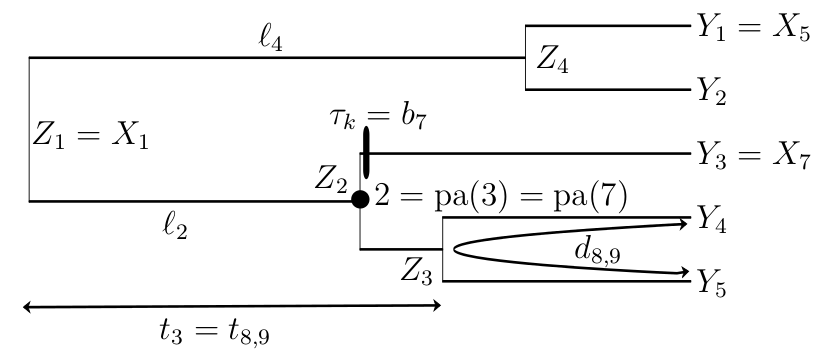
\includegraphics[width=.8\textwidth]{../FIGURES/Notations-BMR15}
  $$
  }
  
%====================================================================
%====================================================================
\end{document}
%====================================================================
%====================================================================

  \begin{tabular}{cc}
    \begin{tabular}{p{.5\textwidth}}
    \end{tabular}
    & 
    \hspace{-.02\textwidth}
    \begin{tabular}{p{.5\textwidth}}
    \end{tabular}
  \end{tabular}

